\documentclass[12pt]{article}
\usepackage{comment} % enables the use of multi-line comments (\ifx \fi) 
\usepackage{lipsum} %This package just generates Lorem Ipsum filler text. 
\usepackage{fullpage} % changes the margin
\usepackage{graphicx}
\usepackage{float}



\title{Scope of Work for Movie Classification Project}
\date{\vspace{-10ex}}

\begin{document}

\maketitle
\noindent
Prepared by Group \#18 \\
Jiejun Lu, jiejunlu@g.harvard.edu\\
Hongxiang Qiu, qiu@g.harvard.edu\\
Weidong Xu, wxu@g.harvard.edu\\
Zeyu Zhao, zeyu\_zhao@g.harvard.edu


\section*{Problem Statement and Background}
In this project we are going to make a machine learning pipeline from scratch to solve the problem of multi-modal genre classification for movies using their posters and/or plot descriptions.\\

\noindent
Project outline:
\begin{itemize}
  \item Scrape a dataset of about 10,000 movies (including their genres, plot descriptions, and posters) from TMDB (or IMDB/Wikipedia).
  \item Perform data pre-processing.
  \item Try conventional machine learning algorithms to build classifiers using text data.
  \begin{itemize}
  	\item Try bag-of-words, word2vec and GloVE word embeddings for movie descriptions.
    \item Try naive-bayes and SVM classifiers for these text features.
  \end{itemize}
  \item Build deep learning algorithms (e.g., RNN) for text data (i.e., plot descriptions).
  \item Build deep learning algorithms (e.g., CNN) for visual data (i.e., posters).
\end{itemize}

\section*{Literature Review}
\subsection*{Conventional machine learning algorithms for NLP}
The first step is usually to apply word embedding techniques to data. Typical word representations include bag-of-words, word2vec \cite{word2vec} and GloVE \cite{GloVE}. We will try multinomial naive bayes and SVM on the processed features.

\subsection*{Deep learning models for NLP}
LSTM (long short-term memory recurrent neural network) has shown remarkable performance in language modeling due to its capability of addressing long-term dependency problem of RNN \cite{LSTM}. C-LSTM, which uses CNN to extract a sequence of higher-level phrase representations and feed into a LSTM to obtain the sentence representation, has been demonstrated to outperform both CNN and LSTM on sentiment classification and question classification tasks \cite{C-LSTM}. Here we plan to apply C-LSTM to the movie genre classification problem.

\subsection*{Deep learning models for computer vision}
It's hard to train a good neural network for posters from the scratch. We need (1) a large dataset and (2) a good architecture design. As suggested in Stanford CS231n course, transfer learning would make our life easier \cite{cs231n}. Since convolution layers can represent general abstract features of an image, we can fix convolution layers of some pre-trained network and re-train the fully connected layers for our new task. VGG16 is a well-trained neural network on ImageNet and its convolution layers are often used for new tasks like segmentation and detection \cite{VGG16}. For poster recognition, we plan to use transfer learning with VGG16's convolution layers.

\section*{Available resources/data}
\begin{itemize}
  \item TMDB: A free, open-source dataset of movie information. We can get movie genres, plot descriptions, and posters by using the python library "tmdbsimple" to make API calls.
  \item IMDB: The standard database for movie information. We can get movie genres, and plot descriptions by using the python library "imdb" to make API calls.
  \item Wikipedia: We can scrape plot descriptions for most movies from their wikipedia pages.
\end{itemize}

\section*{Preliminary EDA}
First, we scraped top 1000 movies from TMDB and the corresponding movies in IMDB, and plotted the movie genre distributions (Figure \ref{fig:eda01}). It turns out the movie genre distributions from 2 databases are very similar.\\

\noindent
Next, we scraped all 361,622 movies from TMDB, and investigated the genre distribution (Figure \ref{fig:eda02}). The distribution is different from that of top 1000 movies, indicating variance in the popularity of different genres. Besides, we plotted the histogram of plot description (i.e., "overview") lengths (Figure \ref{fig:eda03}). Most overviews from TMDB are not long, and the length doesn't seem to vary much, suggesting the feasibility of applying C-LSTM.

\noindent
Finally, we plan to scrape posters of movies in recent years from TMDB.

\begin{figure}[H]
\centering
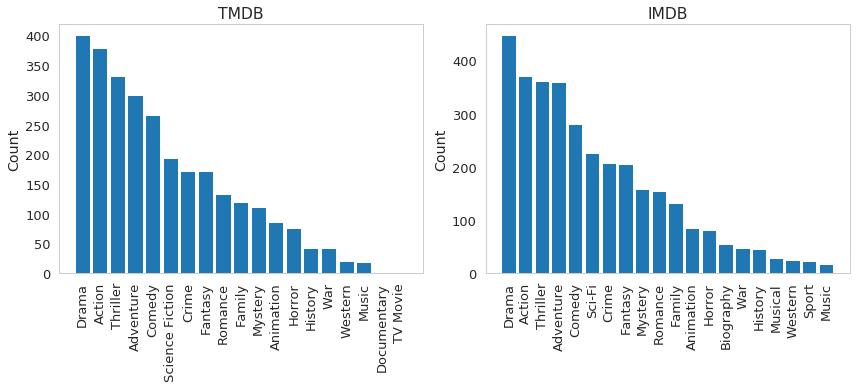
\includegraphics[height=0.4\textwidth]{eda01.png}
\caption{\label{fig:eda01}The movie genre distributions for top 1000 movies in TMDB and the corresponding movies in IMDB.}
\end{figure}
\begin{figure}[H]
\centering
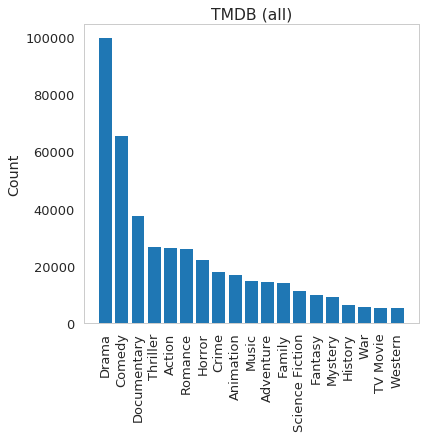
\includegraphics[height=0.4\textwidth]{eda02.png}
\caption{\label{fig:eda02}The movie genre distribution for all 361,622 movies in TMDB.}
\end{figure}
\begin{figure}[H]
\centering
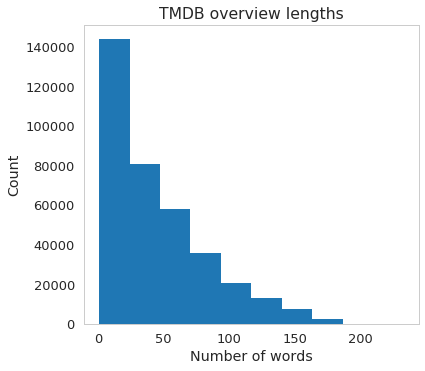
\includegraphics[height=0.4\textwidth]{eda03.png}
\caption{\label{fig:eda03}The movie genre distribution for all 361,622 movies in TMDB.}
\end{figure}

\begin{thebibliography}{9}
\bibitem{word2vec} Tomas Mikolov, Ilya Sutskever, Kai Chen, Greg S Corrado, and Jeff Dean. Distributed representations
of words and phrases and their compositionality. \emph{Advances in neural information
processing systems}, 2013.
\bibitem{GloVE} Jerey Pennington, Richard Socher, and Christopher Manning. Glove: Global vectors for
word representation. \emph{Proceedings of the 2014 conference on empirical methods in natural language
processing (EMNLP)}, 2014.
\bibitem{ML} Spandan Madan. Spandan-Madan/DeepLearningProject: First release of the Deep Learning
Project (https://spandan-madan.github.io/DeepLearningProject/), 2017.
\bibitem{LSTM} Martin Sundermeyer, Ralf Schluter, and Hermann Ney. LSTM Neural Networks for Language Modeling. \emph{INTERSPEECH-2012}, 2012.
\bibitem{C-LSTM} Chunting Zhou, Chonglin Sun, Zhiyuan Liu, and Francis C.M. Lau. A C-LSTM Neural Network for Text Classification. \emph{arXiv:1511.08630}, 2015.
\bibitem{cs231n} Fei-Fei Li, Justin Johnson, and Serena Yeung. CS231n: Convolutional Neural Networks for Visual Recognition (http://cs231n.github.io/transfer-learning/).
\bibitem{VGG16} Karen Simonyan, and Andrew Zisserman. Very Deep Convolutional Networks for Large-Scale Image Recognition. \emph{arXiv:1409.1556}, 2015.
\end{thebibliography}

\end{document}
